%======================================================================
\chapter{System Architecture}
\label{ch: Chapter2}
%======================================================================

%----------------------------------------------------------------------
\section{System Block Diagram}
%----------------------------------------------------------------------
The overall system architecture of this project consists of two subsystems which are the Mobile Cart and the Remote Target, which is held by the user or customer, as shown in \autoref{fig:sys_block_diag}. The proposed smart robotic cart is a wheeled robot that sends and receives radio signals to follow the remote target which acts as the beacon for the robotic cart system.

\vspace*{12pt}
\noindent

The high-level system block diagram of the proposed robotic cart (prototype) is shown in \autoref{fig:sys_block_diag}. There are four inputs to the proposed cart system. The robotic cart is supplied power through a battery that is mounted in the chassis of the robotic cart. There will be an on/off switch to allow the system to be powered down when not in use. The motion of the cart is dependent on the motion of the remote. A stretch goal for the project are mode selection buttons that allow the user to put the robotic cart system into different operating modes.

\vspace*{12pt}
\noindent

The main output of the system is the position trajectory of the robotic cart in its environment. When the user moves with the remote, the cart is designed to follow the user. The other output of the robotic cart system is a status indication in the form of LED lights. These lights will be used to notify the user of the status of the robotic cart.

\begin{figure}[!h]
    \centering
    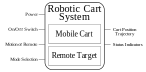
\includegraphics[scale=0.9]{figs/system_block_diagram_2}
    \caption{System level block diagram detailing inputs and outputs to the
      mobile cart system.}
	\label{fig:sys_block_diag}
\end{figure}


%----------------------------------------------------------------------
\section{Subsystem Block Diagrams}
%----------------------------------------------------------------------
The Mobile Cart and the Remote Target subsystems are two separate operations within the robotic cart system that run simultaneously. The two subsystems communicate with one another by relaying radio messages between them. The first block diagram is of the Remote Target subsystem shown in \autoref{fig:remote_block_diag}. Of the two subsystems the Remote Target is the simplest since it only requires an XBee module attached to a 7.4 volt Li-Po battery with a voltage regulation circuit since the XBee has a smaller input voltage of 3.3 volts.

\begin{figure}[h!]
  \centering
  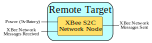
\includegraphics[scale=0.9]{figs/remote_target_block_diagram}
  \caption{Remote Target block diagram}
  \label{fig:remote_block_diag}
\end{figure}

\vspace*{12pt}
\noindent
The Mobile Cart subsystem block diagram is shown in \autoref{fig:mobile_block_diag}. The cart requires a power source, which will be a Li-Po battery since the Li-Po works well with powering the embedded computer (BeagleBone Blue). The power to the subsystem will be toggled by an on/off switch located on the chassis of the robotic cart. The mode selection buttons for changing the operating mode of the robotic cart is a stretch goal of the project and will be implemented on the cart if we have time. The final input to the mobile cart subsystem is the XBee network messages received from the remote target.

\vspace*{12pt}
\noindent
There are three outputs of the mobile cart subsystem. The first is the wheel velocities that move the cart. There will also be LEDs to indicate the status of the system to the user. Lastly, the cart will send radio messages to the remote target by means of a parabolic array of XBee radio modules.

\begin{figure}[h!]
  \centering
  \includegraphics[scale=0.82]{figs/mobile_cart_block_diagram}
  \caption{Block diagram showing the subsystem-level components of the proposed robotic cart.}
  \label{fig:mobile_block_diag}
\end{figure}


%----------------------------------------------------------------------
\section{System Components}
%----------------------------------------------------------------------
There are several components that are required for the mobile cart system. Although some of these parts are available in the Bradley University laboratory, other parts must be purchased. The parts that exist in the lab are shown in \autoref{tab:Partslablist}. Also, \autoref{tab:Partslist} shows the list of parts that we purchased. The parts compiled in the lists are the required parts needed to build two smart robotic cart systems.

\begin{table}[h!]
  \centering
  \begin{tabular}{c|c}
      \toprule
      \textbf{Quantity} & \textbf{Parts}\\
      \toprule
      2 & Budget Bot Chassis\\
      4 & 10 uF Ceramic Capacitor\\
      4 & LM1117 Regulator\\
      2 & Battery Packs for Budget Bot\\
      8 & 9V Batteries\\
      4 & Solderable PCB Boards\\
      3 & XBee USB Adapter\\
      \bottomrule
      %\multicolumn{2}{r|}{\textbf{Total}} & \$ 562.34\\
      %\bottomrule
  \end{tabular}
  \caption{Parts Available in Laboratory}
  \label{tab:Partslablist}
\end{table}

\begin{table}[h!]
  \centering
  \begin{tabular}{c|c|c}
    \toprule
    \textbf{Quantity} & \textbf{Parts} & \textbf{Price}\\
    \toprule
    4 & Pololu 37D Metal Gear motor 4751 & \$ 39.95\\
    12 & XBee S2C Module & \$ 23.10\\
    10 & XBee Adapter Board & \$ 4.99\\
    2 & Twotrees 4 Lead Nema 17 Stepper Motor & \$ 9.99\\
    1 & 4-Pin JST SH Connector - 20 Pack & \$ 7.99\\
    1 & 6-Pin JST SH Connector - 10 Pack & \$ 9.99\\
    1 & Aluminum Foil Tape - 2 in x 5 yd & \$ 6.05\\
    \bottomrule
    \multicolumn{2}{r|}{\textbf{Total}} & \$ 562.34\\
    \bottomrule
  \end{tabular}
  \caption{Purchased parts for the Robotic Cart Project}
  \label{tab:Partslist}
\end{table}

\vspace*{12pt}
\noindent
The main components for this project are the Budget Bot Chassis (\autoref{fig:budgetBotChassis}), the BeagleBone Blue embedded computer (\autoref{fig:beagleboneBlue}), and the XBee S2C Modules (\autoref{fig:XBeeModule}). Another major component is the reflector array that will be used to directionally receive the RF signals from the remote target that is with the user.

\begin{figure}
  \centering
  \begin{minipage}[t]{0.32\textwidth}
    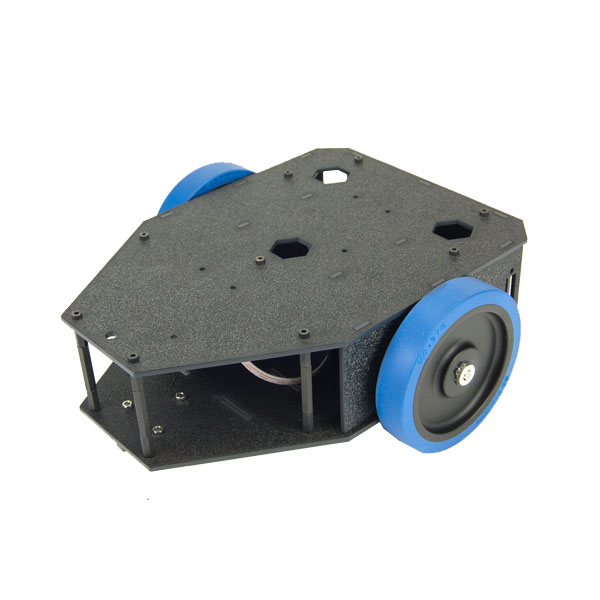
\includegraphics[width=1\textwidth]{figs/img/budgetbot_chassis}
    \captionsetup{width=\textwidth}
    \caption{Budget Bot Chassis}
    \label{fig:budgetBotChassis}
  \end{minipage}%
  \begin{minipage}[t]{0.32\textwidth}
    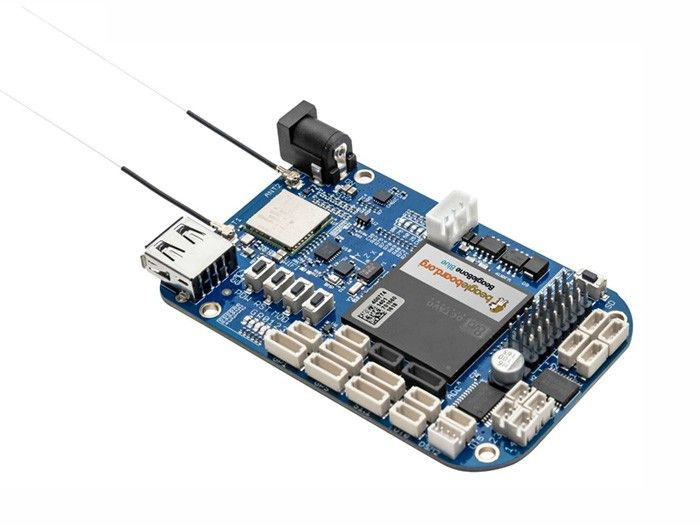
\includegraphics[width=1\textwidth]{figs/img/beaglebone_blue}
    \captionsetup{width=\textwidth}
    \caption{BeagleBone Blue}
    \label{fig:beagleboneBlue}
  \end{minipage}
  \begin{minipage}[t]{0.32\textwidth}
    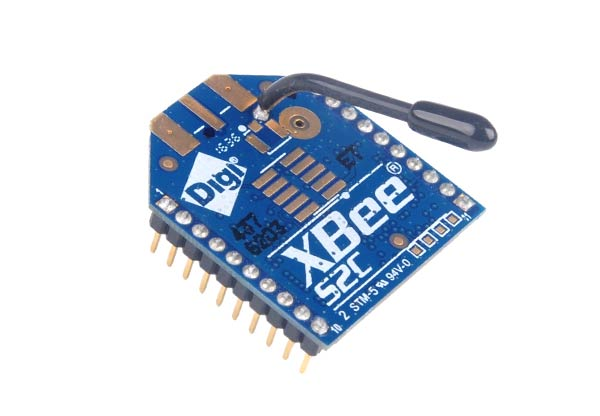
\includegraphics[width=1\textwidth]{figs/img/Xbee-S2C-Module}
    \captionsetup{width=\textwidth}
    \caption{XBee S2C Module}
    \label{fig:XBeeModule}
  \end{minipage}
\end{figure}

\vspace*{12pt}
\noindent
The reflector array will be mounted on top of the cart with a stepper motor. There are two reflector designs that we will be evaluating in this project. The first, shown in \autoref{fig:parabolodialReflector}, is a paraboloidal reflector which maximizes the signal strength of the signals that come into the reflector perpendicularly. Since the remote will be carried by the user, it is likely that it will be positioned at a higher altitude than the reflector array. The paraboloidal reflector design may not be able to pick up the signals from the remote as well because of this. To solve this problem, we designed a combination parabolic/paraboloidal reflector, as shown in \autoref{fig:parabolicReflector}. The lower half of this reflector is paraboloidal in shape to limit the signals coming from below. The upper part of the reflector is strictly parabolic. This shape focuses the signals in the horizontal plane, but allows signals from above to still be received. We plan to construct both of these reflector designs by 3D printing the frames, then lining them with reflective foil tape. Both models will then be tested to determine which design works better.

\begin{figure}[h!]
  \centering
  \begin{minipage}[t]{0.5\textwidth}
    \centering
    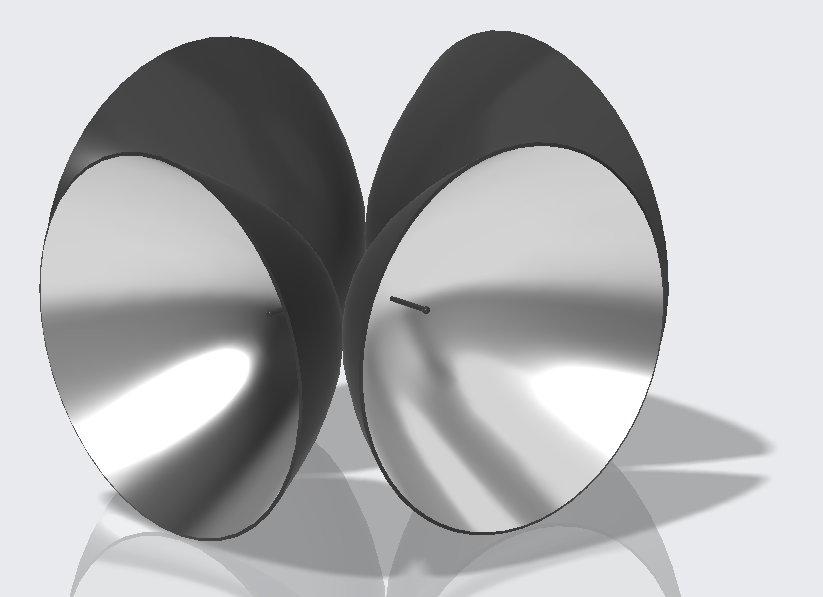
\includegraphics[height=2in]{figs/img/paraboloidalReflector}
    \captionsetup{width=\textwidth, justification=raggedright}
    \caption{Paraboloidal Reflector Model}
    \label{fig:parabolodialReflector}
  \end{minipage}
  \begin{minipage}[t]{0.4\textwidth}
    \centering
    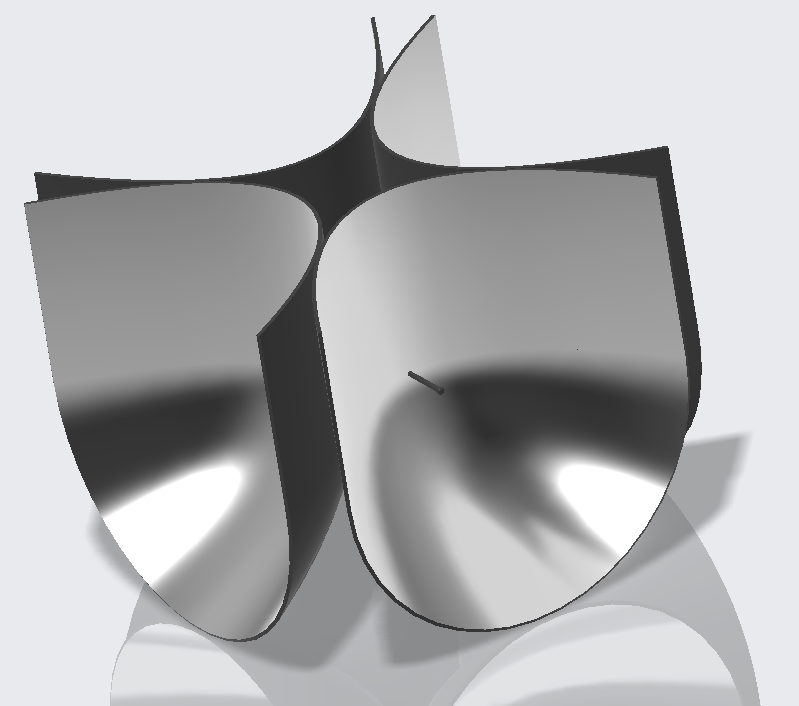
\includegraphics[height=2in]{figs/img/parabolicReflector}
    \captionsetup{width=\textwidth, justification=raggedright}
    \caption{Combined Parabolic/Paraboloidal Reflector}
    \label{fig:parabolicReflector}
  \end{minipage}
\end{figure}

\subsection{Operation of Mobile Cart System}
The mobile cart will be controlled by a central embedded computer which is the BeagleBone Blue since it is ideal in robotics control. Two DC motors will be used to drive wheels and move the cart. Five XBee modules on the cart will be used to allow communication with the remote target. One of these radio sensors will be mounted on top of the cart to broadcast in all directions. The other four sensors will be placed inside parabolic reflectors at right angles to each other. This sensor array will be mounted on a stepper motor to allow rotation.


%%% Local Variables:
%%% mode: latex
%%% TeX-master: "../finalReportMainV1"
%%% End: